%!TEX root = paper/paper.tex
\section{Introduction}
\begin{figure}[t]
\small{
\centering
\begin{subfigure}[t]{0.48\linewidth}
    \begin{tabular}{cc}
    %
    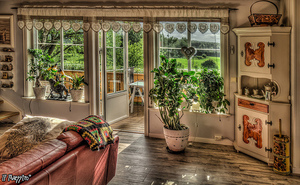
\includegraphics[width=.43\linewidth]{../../figures/flickrDatasetExamples/used/resized/hdr.jpg} &
    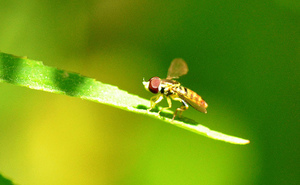
\includegraphics[width=.43\linewidth]{../../figures/flickrDatasetExamples/used/resized/macro.jpg} \\
    HDR & Macro \\
    %
    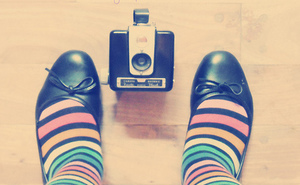
\includegraphics[width=.43\linewidth]{../../figures/flickrDatasetExamples/used/resized/vintage.jpg} &
    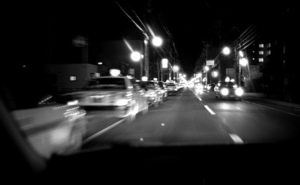
\includegraphics[width=.43\linewidth]{../../figures/flickrDatasetExamples/used/resized/noir.jpg} \\
    Vintage & Noir \\
    %
    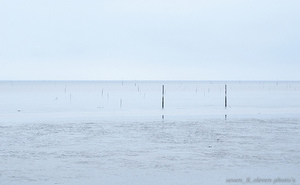
\includegraphics[width=.43\linewidth]{../../figures/flickrDatasetExamples/used/resized/minimal.jpg} &
    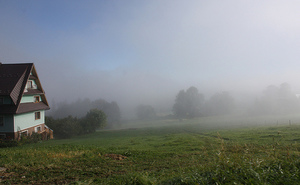
\includegraphics[width=.43\linewidth]{../../figures/flickrDatasetExamples/used/resized/hazy.jpg} \\
    Minimal & Hazy \\
    %
    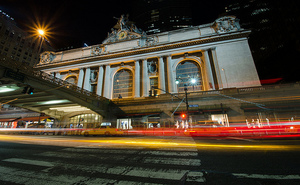
\includegraphics[width=.43\linewidth]{../../figures/flickrDatasetExamples/used/resized/long_exposure.jpg} &
    
\includegraphics[width=.43\linewidth]{../../figures/flickrDatasetExamples/used/resized/romantic.jpg} \\
    Long Exposure & Romantic \\
    \end{tabular}
    \caption{
        Flickr Style: 80K images covering 20 styles.
    }\label{fig:flickr_style_examples}
\end{subfigure}%
\hspace{2em}%
\begin{subfigure}[t]{0.48\linewidth}
    \begin{tabular}{cc}
    %
    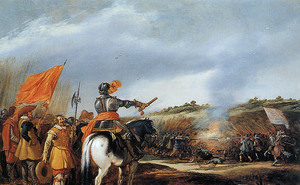
\includegraphics[width=.43\linewidth]{../../figures/wikipaintingsDatasetExamples/used/resized/baroque-0.jpg} &
    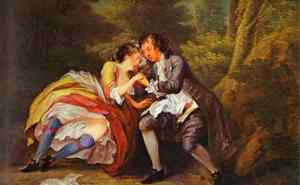
\includegraphics[width=.43\linewidth]{../../figures/wikipaintingsDatasetExamples/used/resized/roccoco-0.jpg} \\
    Baroque & Roccoco \\
    %
    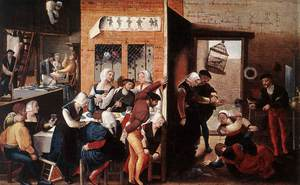
\includegraphics[width=.43\linewidth]{../../figures/wikipaintingsDatasetExamples/used/resized/northern_renaissance-0.jpg} &
    % NOTE: ukiyoe-0 is messing up for unknown reason
    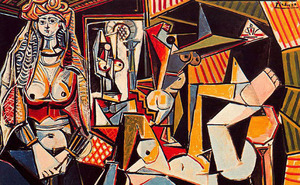
\includegraphics[width=.43\linewidth]{../../figures/wikipaintingsDatasetExamples/used/resized/cubism-0.jpg} \\
    Northern Renaissance & Cubism \\
    %
    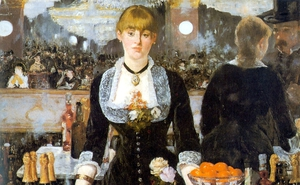
\includegraphics[width=.43\linewidth]{../../figures/wikipaintingsDatasetExamples/used/resized/impressionism-0.jpg} &
    % NOTE: post-impressionism was messing up until I output it as png
    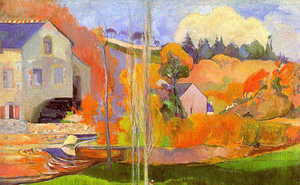
\includegraphics[width=.43\linewidth]{../../figures/wikipaintingsDatasetExamples/used/resized/post_impressionism-0.jpg} \\
    Impressionism & Post-Impressionism \\
    %
    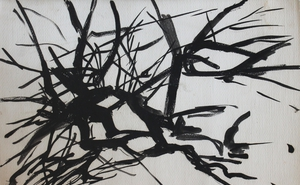
\includegraphics[width=.43\linewidth]{../../figures/wikipaintingsDatasetExamples/used/resized/abs_expressionism-0.jpg} &
    
\includegraphics[width=.43\linewidth]{../../figures/wikipaintingsDatasetExamples/used/resized/color_field-0.jpg} \\
    Abs. Expressionism & Color Field Painting \\
    \end{tabular}
    \caption{
        Wikipaintings: 85K images for 25 art genres.
    }\label{fig:wikipaintings_style_examples}
\end{subfigure}
}
\caption{
    Typical images in different style categories of our datasets.
}\label{fig:style_examples}
\end{figure}


Deliberately-created images convey meaning, and \textit{visual style} is often a significant component of image meaning.
For example, a political candidate portrait made in the lush colors of a Renoir painting tells a different story than if it were in the harsh, dark tones of a horror movie.
Distinct visual styles are apparent in art, cinematography, advertising, and have become extremely popular in amateur photography, with apps like Instagram leading the way.
While understanding style is crucial to image understanding, very little research in computer vision has explored visual style.

Although is it very recognizable to human observers, visual style is a difficult concept to rigorously define.
% It depends on choices of colors, lighting, composition, scene objects, and optical techniques, and might suggest specific moods and genres.
Most academic discussion of style has been in an art history context, but the distinctions between, say, Rococo versus pre-Rafaelite style are less relevant to modern photography and design.
There has been some previous research in image style, but this has principally been limited to recognizing a few, well-defined optical properties, such as depth-of-field.

We define several different \textit{types} of image style, and gather a new, large-scale dataset of photographs annotated with style labels.
This dataset embodies several different aspects of visual style, including photographic techniques  (``Macro,'' ``HDR''), composition styles (``Minimal,'' ``Geometric''), moods (``Serene,'' ``Melancholy''), genres (``Vintage,'' ``Romantic,'' ``Horror''), and types of scenes (``Hazy,'' ``Sunny'').
These styles are not mutually exclusive, and represent different attributes of style.
We  also gather a large dataset of visual art (mostly paintings) annotated with art historical style labels, ranging from Renaissance to modern art.
\autoref{fig:style_examples} shows some samples.

We test existing classification algorithms on these styles, evaluating several state-of-the-art image features.
Most previous work in aesthetic style analysis has  used hand-tuned features, such as color histograms.
We find that deep convolutional neural network (CNN) features perform best for the task.
This is surprising for several reasons: these features were trained on object class categories (ImageNet), and many styles appear to be primarily about color choices, yet the CNN features handily beat color histogram features.
This leads to one conclusion of our work: mid-level features derived from object datasets are generic for style recognition, and superior to hand-tuned features.

We compare our predictors to human observers, using Amazon Mechanical Turk experiments, and find that our classifiers predict Group membership at essentially the same level of accuracy as Turkers.
We also test on the AVA aesthetic prediction task \cite{Murray-CVPR-2012}, and show that using the ``deep'' object recognition features improves over the state-of-the-art results.

\paragraph{Applications and code.}
First, we demonstrate an example of using our method to search for images by style.
This could be useful for applications such as product search, storytelling, and creating slide presentations.
In the same vein, visual similarity search results could be filtered by visual style, making possible queries such as ``similar to this image, but more Film Noir.''
Second, style tags may provide valuable mid-level features for other image understanding tasks.
For example, there has increasing recent effort in understanding image meaning, aesthetics, interestingness, popularity, and emotion (for example, \cite{Gygli-ICCV-2013,Isola-CVPR-2011,joo2014,khosla2014}), and style is an important part of meaning.
Finally, learned predictors could be a useful component in modifying the style of an image.

All data, trained predictors, and code (including results viewing interface) are available at \url{http://sergeykarayev.com/recognizing-image-style/}.
